% 2023年北京高考数学第16题：四面体P-ABC
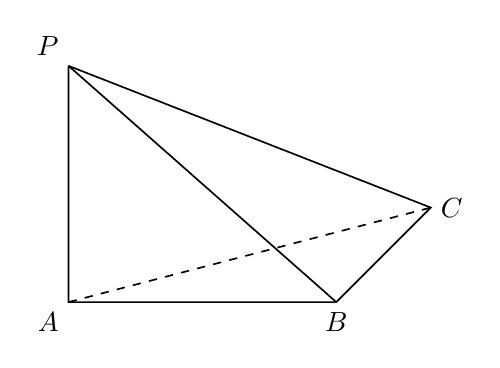
\begin{tikzpicture}[>=stealth,line width=0.6pt,font=\normalsize]
  \coordinate (A) at (0,0);
  \coordinate (B) at (3.4,0);
  \coordinate (C) at (4.6,1.2);
  \coordinate (P) at (0,3.0);

  % 实线边
  \draw (P) -- (A) -- (B) -- (C) -- (P);
  \draw (P) -- (B);

  % 虚线底面边
  \draw[dashed] (A) -- (C);

  % 顶点标注
  \node[above left] at (P) {$P$};
  \node[below left] at (A) {$A$};
  \node[below] at (B) {$B$};
  \node[right] at (C) {$C$};
\end{tikzpicture}
